\chapter{INTRODUÇÃO}
\label{cap:introdução}

Este catapítulo apresenta uma visão geral do problema pesquisado bem como as soluções encontradas para tal, juntamente com os materiais e metologias empregados na busca da solução.

\section{Justificativa}

\subsection{Introdução a Teste de Software}
A construção de softwares em ampla maioria dos casos, usufruem dos planejados e estudados processos da engenharia de software objetivando uma escalabilidade desse processo para tentar se evitar erros, seja na implementação técnica dos algorítimos ou em errôneas interpretações casuais por parte de analises humanas equivocadas. Existem diversas técnicas para testes de software, mas em sua generalidade, trabalham sobre a ideia de avaliar dado um conjunto de possíveis entradas, a saída processada de tais conjuntos através das permutações de estados que o software em questão pode assumir.

Denota-se um problema intratável avaliar todas as possíveis entradas para um software, haja visto a cardinalidade de certos conjuntos de entrada, então, muitas técnicas exprimem a estratégia de se selecionar subconjuntos contidos no conjunto de entradas possíveis, tal que seus elementos pertinentes representem o conjunto maior em questão.

Mostra-se recente a atenção para a importância da adoção de tais procedimentos por empresas do ramo, visando uma redução em problemas com consumidores e manutenção pós produção desses sistemas, uma vez em que testes podem auxiliar na avaliação do funcionamento escalável de todos os módulos e componentes do presente software.

\begin{figure}[!htb][H]
\centering
\caption{Diferentes comportamentos para um mesmo caso de teste} %legenda
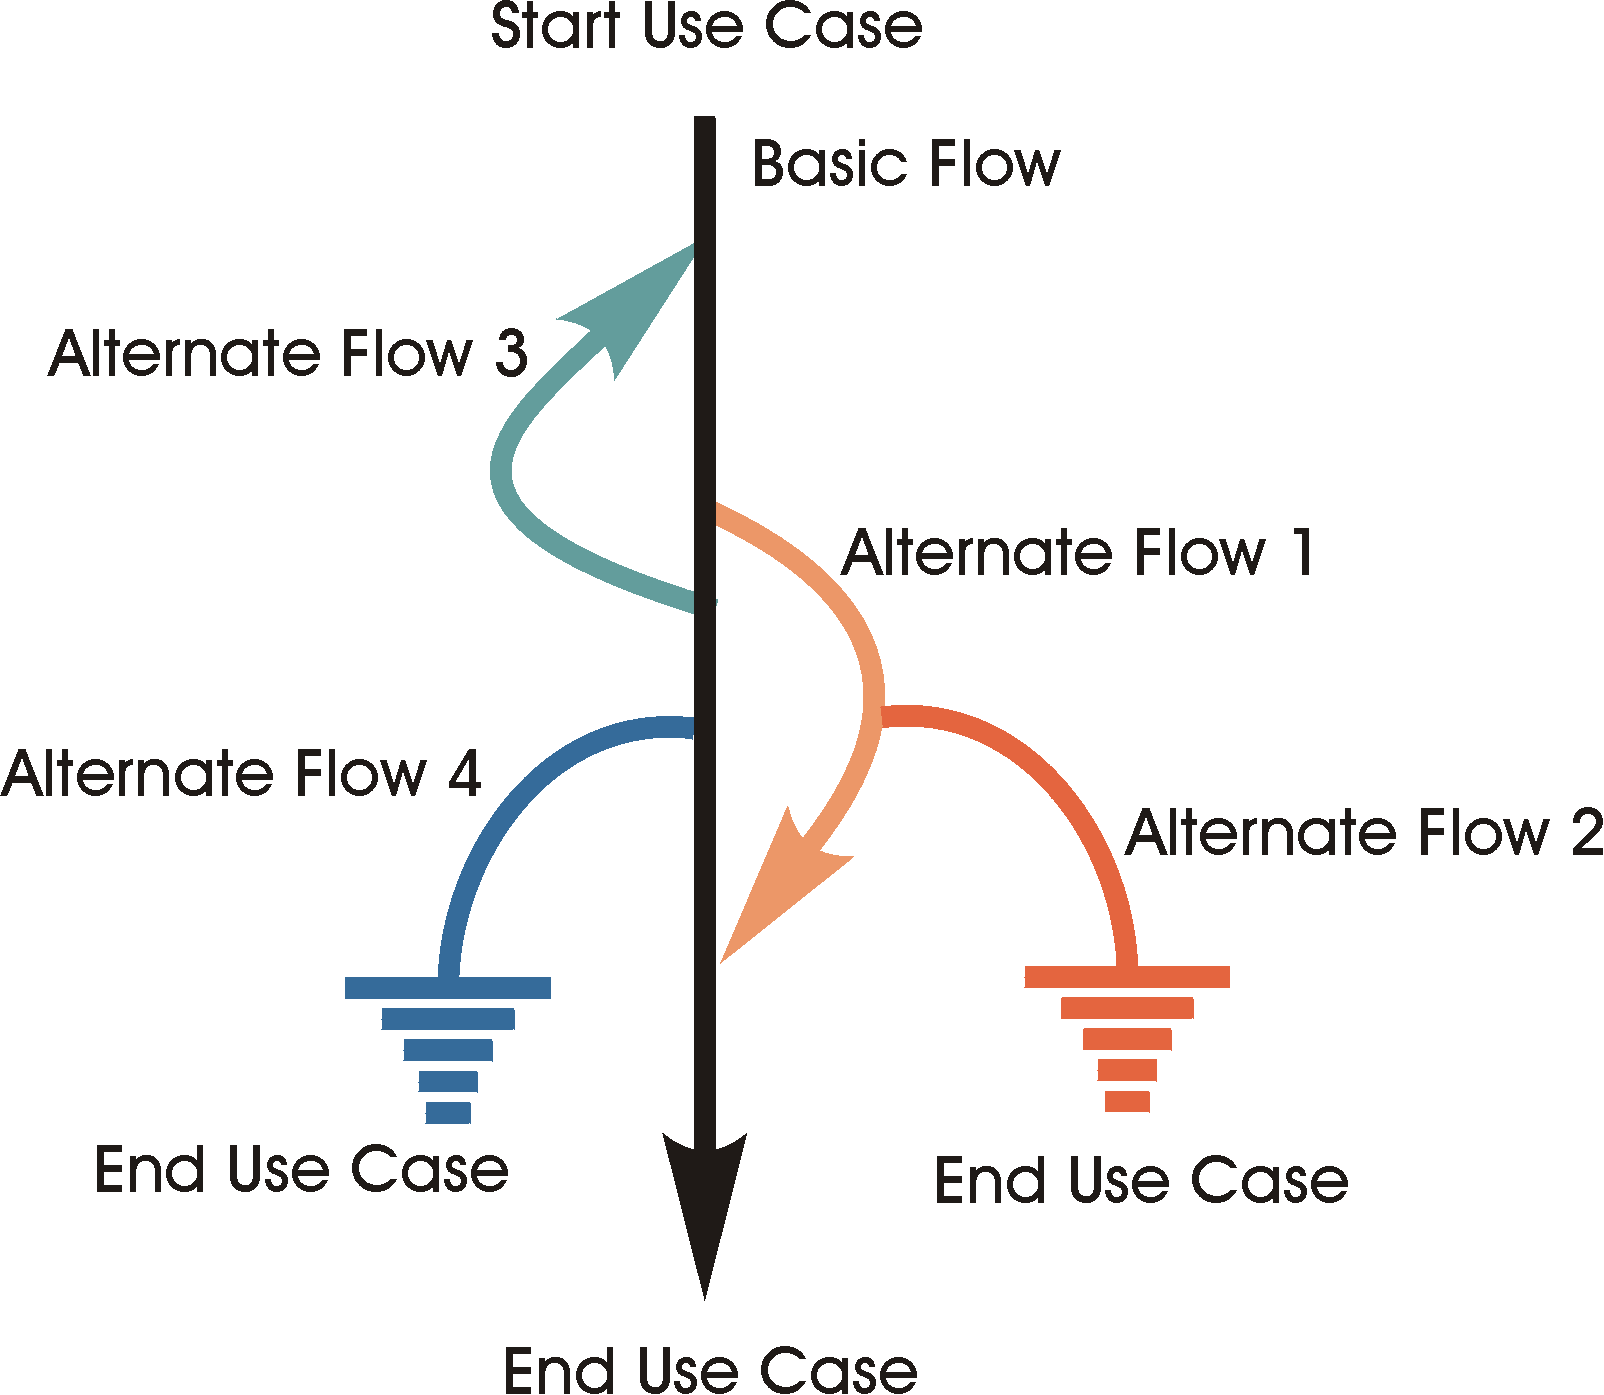
\includegraphics[scale=0.1]{02}\\  % o 0.9 indica 90% do tamanho original
{\small Fonte: Guideline: Test Case	- http://www.michael-richardson.com} %Fonte da imagem
\label{fig:exemplo} %rotulo para refencia
\end{figure}


\subsection{Seleção de Casos de Teste}
Como supracitado, a seleção desse subconjunto ou seleção de casos de teste, é praticada por seres humanos, e por consequência a tal, são suscetíveis a falhas humanas, em decorrência de diversos fatores como: Equívoca interpretação sobre requisitos extraídos de um documento de requisitos do software, relação entre experiencia técnica de tal testador para com formalidade da expressão de tais requisitos, elaboração erronia de tais requisitos no contato entre fornecedor e consumidor do produto, dentre outros.

Há de ressaltar que aplicação de testes de software não garante a corretude de um software ou algorítimo, onde como citado, necessita-se da aplicação de testes para todos os elementos pertencentes ao conjunto de possíveis entradas para o software, mas busca uma minimização de problemas ocasionais de tais falhas e uma maior segurança ao usuário final.

\subsection{Processamento de Línguas Naturais}
Essa área é responsável por compreender os mais variados aspectos e toda a estrutura gramatical de um idioma e a língua humana por meio de algorítimos para uma posterior abordagem das informações obtidas seja para reconhecimento e formulação de bases de conhecimento, automação de tarefas dependentes de avaliação ou interferência humana dentre outras inúmeras aplicações da tecnologia e ciência.
Com foco no presente projeto, discute-se o processamento textual de requisitos elicitados diretamente de um cliente como parte de um mercado consumidor e a abstração de informações com base em conhecimentos da Engenharia de Software para a construção de uma estrutura de um software e a seleção de casos de teste.

Para processar corpus textuais construídos em língua humana, é preciso reconhecer as estruturas gramaticais e sintáticas do respectivo idioma e processa-las segundo algum algorítimo de PLN que efetua avaliações probabilísticas sobre a sentença e sua composição para determinar classes gramaticais e aferir semanticamente qual o sentido do que está sendo compreendido, tudo isso atraves de arvores sintáticas como demonstrado a seguir:

\begin{figure}[!htb][H]
\centering
\caption{Árvore sintática da sentença em Inglês} %legenda
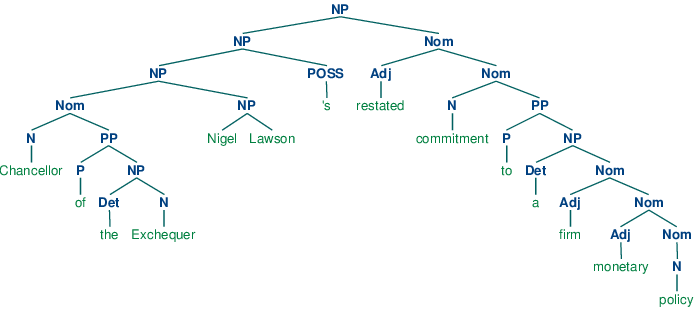
\includegraphics[scale=0.5]{01}\\  % o 0.9 indica 90% do tamanho original
{\small Fonte: Natural Language Toolkit - http://www.nltk.org} %Fonte da imagem
\label{fig:exemplo} %rotulo para refencia
\end{figure}

\section{Problema da Pesquisa}
Em países pertencentes ao polo de produção centralizada tecnológica, é amplo a gama de opções de ferramentas para auxiliar o papel do testador dentro das empresas, mas no cenário brasileiro, opções ainda são escassas. Essa escassez de ferramentas disponíveis para as empresas brasileiras de tecnologia da informação, reduzem a competitividade do país no setor bem como amplia os custos referente a cadeia de produção de softwares no Brasil.

A elevação dos custos supracitado, ainda pode decorrer em uma maior negligência por parte de tais corporações quanto a qualidade de sua produção, uma vez em que o alto custo empregado no processo de teste dos softwares pode não ser contemplado, aumentando assim, os riscos de insatisfação do mercado consumidor ou problemas em outras cadeias de produção, cujo é um componente agregado, o software em questão.

\section{Objetivo}
O objetivo da pesquisa do presente projeto busca avaliar de forma sistemática, a viabilidade da adoção para o idioma português de ferramentas de Processamento de Língua Natural existentes e desenvolvidas para o idioma Inglês, onde tangente a tal adoção, seja necessário mudanças pontuais nas estruturas de processamentos destes mecanismos para que seu funcionamento seja voltado para o idioma Português do Brasil.

Em futuras etapas de desenvolvimento do projeto, propõe-se a construção de uma ferramenta capaz de, a partir da entrada de um documento de requisitos e especificações de software, realizar a extração de informações necessárias para a construção e seleção de casos de teste, onde em seguida, seja capaz de gerar diagramas de sequencia, classe, dentre outros que beneficiem o processo de construção em modelo UML, a geração automatizada de maquinas de estado para que os testes extraídos e selecionados, possam ser executados de forma também automática, produzindo os resultados que auxiliaram o trabalho do testador e reduzirá a quantidade de falhas de software decorrentes de interferência humana, onde tal ferramenta para o idioma Português, ampliará a gama de opções disponíveis ao mercado brasileiro voltado para empresas de produção de software.

%%%%%%%%%%%%%%%%%%%%%%%%%%%%%%%%%%%%%%%%%%%%%%%%%%%%%%%%%%%%%
%O objetivo deste documento é apresentar o uso básico da classe {\tt uflamon} para a elaboração de monografias da UFLA utilizando a linguagem de marcação \LaTeX\ \cite{Lamport1994}.  A maioria dos comandos (macros) e ambientes das classes básicas da linguagem é válida também nessa classe, que é estendida com comandos para confecção da capa, páginas de rosto, dedicatórias, etc.

%A classe foi baseada inicialmente nas normas da PRPG/UFLA para produção de TCC \cite{PRPG2006}. Essas normas foram posteriormente atualidas, de maneira geral pela UFLA, para a produção de monografias, dissertações e teses \cite{BIB2010}.  A versão atual da {\tt uflamon} reflete a última versão da norma \cite{UFLA:2015}.

%Este texto, que objetiva apresentar um exemplo de uso da classe  {\tt uflamon}, encontra-se organizado como se segue. O Capítulo~\ref{cap:elementos} apresenta exemplos de inserção de figuras, tabelas, equações e demais elementos explicativos. O Capítulo~\ref{cap:conclusao} apresenta comentários e observações finais. Por fim, o Apêndice~\ref{cap:apendice} mostra como elaborar um apêndice simples.